\documentclass[main.tex]{subfiles}
\begin{document}
\section{Question 2}
Create a child process. Let the parent sleeps of 5 seconds and exits. Can the
child send SIGINT to its parent if exists and kill it? Verify with a sample
program.

\lstinputlisting[style=codeStyleC]{listings/2.c}
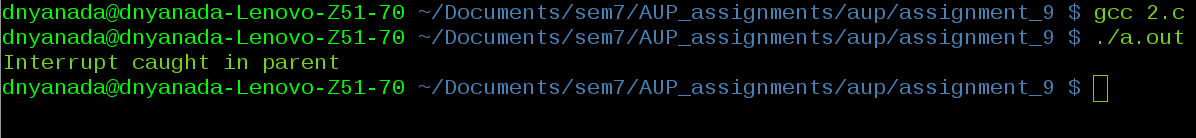
\includegraphics[width=\textwidth]{figures/2_output.png}

Yes, the child can send a SIGINT and kill the parent. This can be verified by
registering a handler in parent to catch SIGINT.
\end{document}
